\part{Introduction}

\chapter{Introduction and theoretical background}

What has been one of the main dangers humanity has faced throughout its history? The first answers that can be given are war or climate change, but there is another great threat that has severely affected the lives of almost all the population on earth: disease and epidemic. There is not a period neither nowadays nor in the past in which illness has not influenced our lives. 

Looking to the past the consequences of the epidemic on the population were worse than today because of the lack of knowledge about medical science and the poor hygienic conditions.  During the bubonic plague of the 14th century, for example, 25 million deaths were reported in Europe out of a population of 100 million. Jews were considered responsible for the illness spread and they began to be persecuted.
Otherwise, in the course of the Americas' colonization, the disease imported by the Europeans was one of the main causes of the genocide of the local population, causing their defeat against the Spanish conquistadores. In fact, diseases like smallpox and cholera were unknown in these countries and native Americans had no antibodies to contrast them. 
Other important epidemics, famous for their consequences were Spanish influenza, Smallpox, Typhus, HIV/AIDS, and the more recent Covid-19. 
It is straightforward to notice the effect that diseases have on our lives.

The development of modern medicine and hygiene can contribute to enhancing the quality of life. An example of this is that only in the last three centuries and just in the most developed countries, like Europe and North America, a significant increase in life expectancy has been observed. Even if mortality is decreased, the modification in social patterns and the development of large cities, have had some consequences: a higher density of population has increased in the $18^{th}$ and $19^{th}$ centuries the frequency and magnitude of epidemics. FIGURA DI QUESTO TREND As it can be seen, even if some improvements in health status were achieved, the presence of new disease potentially escalating in an outbreak is a concrete menace that needs attention and consideration on health policies. 

However, the health status is not the only aspect concerned with a disease. Being sick causes profound modification in our relationship, work, and social life, for example, causing a deterioration of also the social health. 
There is also an economic cost associated with the cure necessary to be healed. Only in a few nations worldwide, is treatment covered free of charge by the state. In the majority, being ill can result in having to sustain high costs, causing people to go into debt or not take care. 
All these effects sum together and influence how populations behave when facing an epidemic. What are the consequences of adopting a certain behavior during a disease outbreak? It's a crucial question and can help to understand how to develop more efficient policies for contrasting epidemics. It is also the question that represents the first objective of study for the present work: can a multidisciplinary-based model be developed, integrating social and epidemiological features and analyzing their mutual relationship during a disease spread? 

Taking a step back, it is important to explain why epidemic models are so important, and how is composed their research field. 

Nowadays, but also in the past when a new disease appears understanding its origin, the biological mechanism under its spread, and comprehending its resistance to existent drugs are examples of crucial aspects to developing a defense against it.
These are part of the epidemiological investigation that aims to collect all the information available to understand what is happening.  
Then epidemiology tries to take a step further by only reconstructing the cause behind the disease development: modeling how can evolve over time. 
 A plethora of different key dimensions were under analysis in this process. For example, genetic resistance, selective pressure of disease on different human communities, and the mechanism underlying the acquisition of immunity. 
\begin{figure}[hbt!]
	\centering
	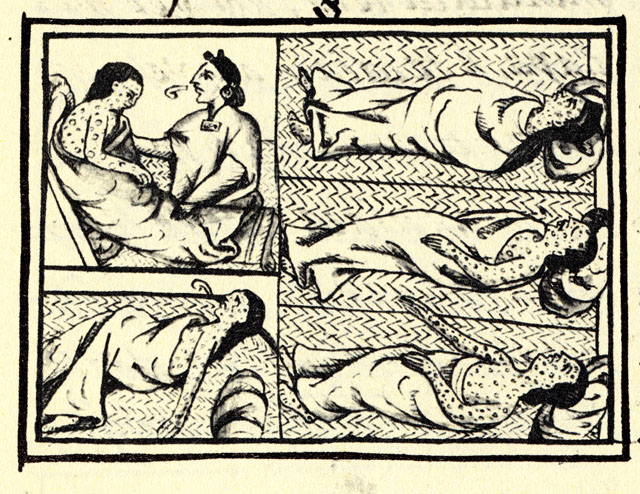
\includegraphics[width=0.4\linewidth]{0_introduction/images_introduction/FlorentineCodex_smallpox}
	\caption[smallpox on native Americans]{Representation of smallpox disease on the Mexican population in the $XIV$ century. Figure from the Florentine Codex \cite{Sahagun1965}. }
	\label{fig:florentinecodexsmallpox}
\end{figure}
There is a lot of interest about this topic both from a scientific perspective and also for public society regulations.
Develop a model that can give us the capability of estimate phenomena like the spread of a disease have a multitude of effects and outcomes on the society.  Social and economic costs are related to every illness, but develop instruments to better understand its impact can avoid the losses of human life and permit to have less serious effect on the society. 
A first simple example, that can help to understand the beneficial effect of study epidemics is the possibility to develop instruments that can permits to consider the specificity of each different disease with "simple" parameters and obtain information like:

\begin{itemize}
	\item is this disease so infective that can cause a pandemic?
	\item what are the threshold conditions that can cause an outbreak? 
\end{itemize}


At a first look the problem can seem simple. Unfortunately, the creation of a model capable of perform an evaluation like the one explained above, suitable for every disease is a problem for which there is not still a solution. 
Every research about the creation of a model that try to represent a real phenomenon must confront with the necessity to simplify, while trying to not loss in accuracy. 
So, in a century of research, many different aspects regarding an epidemic have been considered. The scientist try to catch the most significant ones to develop their model and then figure out if it is capable to give them insights about the considered disease. 
% Qui sarebbe carino iniziare con un discorso che spieghi un po' gli obbiettivi del lavoro 



% ! Ci sta inizialmente concentrarsi sulle epidemie, ma  devi intrudurre anche il secondo macro filone, quello delle opinioni. é uno spin off metodologico del primo, quindi gli stumenti matematici poi sono simili, ma va detta anche questa cosa. E poi sulle opinioni hai visto quante sfumature diverse esistono sul come considerarle e anche questo è da tenere in considerazione. 

\section{Epidemiological theory foundations}

Definition of the theoretical basis and main concepts that will be used in the present work. 
\subsection{ Epidemiologic research historical background}
% Se ti piace l'idea di fare un piccolo excursus storico, va bene. Le info principali sono:
% 1- primo lavoro di Bernoulli
% 2- lavori di Hamer (1906) mass action principle, epidemic description in discrete time 
% 3- Ross, formulation in continous time 
% 4- Kermack and Mc Kendrick (1927) che danno risultato bello perchè introducono "legge" del thresold di una epidemia
% Dopo aver scritto quest'ultimo evento hai il LA per parlare di come funziona un mean field model. 

The research field regarding the development of technique to understand how epidemics can evolve during time has a history starting back in the 20th century. The first important discovery in this field must be attributed to the scientists that find the mechanism used by disease to spread. 
A first innovative work is the one done by John Snow, that during an epidemic of Cholera in London in 1854 successfully determined the source of the infection, even without knowing its etiological agent. Then advancing in the microbiological research is conducted by Pasteur and Koch. They found the etiological agent of disease, enabling the possibility to treat and prevent people from an infection. 
Then, Hamer work in 1906 added a first major theoretical contribution. He formulated a theory about the correlation between the course of an epidemic and the interaction, contact ratio, between susceptible and infectious individuals. It is the so called “mass -action” principle. The number of contacts between these two groups determines the spread rate of the disease. 
This law originally written in discrete time, is then updated in 1908 by Ross, that re-written it  in continuous time. For the first time the problem can be studied using a clearly, well defined mathematical theory. Then the contributions of Kermack and McKendrick in 1927 add another fundamental principle to the modern epidemiology. They formulated a threshold theory explaining which condition can generate the development of an epidemic. The theorem affirms that a certain value must be exceed, depending on the proportion of susceptible and infectious individual. Controlling this value permits to understand if the number of infections will increase, until a peak is reached or if the epidemic is a descendent phase \cite{Mata2021}, \cite{Anderson_82}. 
Their contribution with the mass action principle represents the base for the mean field model theory, that will be presented and analysed in section \ref{subsec:SIR}. 



\subsection{Epidemiological glossary}
To permit a better comprehension of the subject analyzed in the present work a list of principal concepts and terms is presented.

\subsubsection{Micro and Macro parasite}
	The first difference when presenting infection is distinguishing the type of origin that can cause it. An etiological organism responsible for a disease can be divided into microparasite and macroparasite. The former live and reproduce within the host, generating an immune response and the infections caused by them usually have two possible outcomes: death or immunity. Infections origins from them are shorter than the life span of an individual, and so have a transient nature.
\subsubsection{Types of infectious diseases}
Infectious disease is indicated as an illness resulting from the presence of a pathogenic microbial agent. It is possible to distinguish a difference between \textit{transmittable} and \textit{communicable} disease. A transmittable disease can transmitted between persons through unnatural forces. A disease is communicable when the transmission happens directly or indirectly.

\subsubsection{Disease transmission} A disease can spread in different ways: 
	\begin{itemize}
		\item person to person, for example sexual transmission, involving direct or indirect contact.
		\item airborne, through inhalation of infected air.
		\item food or water borne, ingesting contaminated food. 
		\item vector born, the contagion is caused by infected animals.
	\end{itemize}
	Furthermore when the diffusion is among the same generations is called horizontal transmission, while vertical transmission is the one developing between different generations, from parents to children. 
	Zoonosis is the phenomenon in which a disease that starts in an animal species mutates and attacks humans. The opposite can also happen and it is called inverse-zoonosis. 
	
\subsubsection{Epidemic disease} It occurs when there is a disease with a rapid outbreak, in less than a year there is its development and a peak is reached. The illness is confined to a limited region

\subsubsection{Endemic disease} It is a disease that lasts for a long time and requires consideration of its impact on population renewal and in the number of susceptible individuals.

\subsubsection{Pandemic disease} It is an epidemic that diffuses across multiple regions, on a global scale. The severity of the disease also makes a distinction in calling a disease a pandemic. For example, a common cold is diffused in the whole world but is not defined as a pandemic by the WHO (World Health Organization). 

\subsubsection{Incubation, Symptoms, Infected and Infectious}   A person having contact with another infectious individual, can or not become infected. The incubation is the period after being infected in which the infection increases in size or number in the host but does not produce the symptoms, that are the effect of the disease. 

\subsubsection{Outbreak} Is the rapid raise in the number of infected during an epidemic.

\subsubsection{Incidence and prevalence} The first term refers to the number of new cases after a certain period (daily or weekly for example), while prevalence is the proportion of the population affected by a disease in a specific time.

\subsubsection{Immunity and herd immunity} Immunity is protection from a disease gained after having contracted it. It can last forever or vanish after a certain time. New exposure to the virus does not lead to infection. Herd immunity is instead an important phenomenon in which the defense against a disease is due to the majority of the population being immune, thanks to vaccines or surviving it. This majority protects the rest of the population because slows down the diffusion or stops the spread of the illness.

\subsubsection{Virulence and Contagiousness}  Virulence is used to describe how aggressive, harmful, and pathogenic is a biological agent in attacking cells. Contagiousness is referred to an individual and it is used to represent the capability to transmit a disease. 

\subsubsection{Overdispersion and Superspreading} Overdispersion is a term that refers to observing a larger variance than expected from a normal distribution. It is used in statistics to measure superspreading, a circumstance in which there is an anomaly (higher) number of secondary infections.

\subsubsection{CFR, IFR and mortality excess} The case fatality rate is the ratio between the number of deaths due to a specific disease and the total number of confirmed positive cases. It is the likelihood for an infected person to die because of the infection. The infection fatality rate is instead the percentage of people infected with the disease that are expected to die. The two quantities can have a similar value: if every person who contracts the disease and every death attributable to the disease is known and recorded, then the CFR will equal the IFR.
The excess in mortality can be calculated by observing the difference between the total death rate (due to any reason) a month per month in a comparison between a year with an epidemic and one without. 

\subsubsection{Reproduction number $R_0$} It is the fundamental measure of the infectiousness of a disease. It is the average number of secondary infections caused by one infected person in a fully susceptible population. If it is recalculated during the epidemic progression is called $R(t)$, a time-varying reproduction number. Finally exist also the effective reproduction number, describes the average number of secondary infected people during the epidemic (rescaling the value with the true number of susceptible). 


\subsubsection{Incubation period and serial interval} The incubation is the time after exposure in which the disease develops and ends when the infected start to show symptoms. The serial interval is instead the time that exists between two transmissions in a chain of infections. 

%%%%%%%%%%%%%%%%%%%%
\section{Opinion/behaviour glossary}
To establish a framework suitable for developing and understanding behavioral models, the following key concepts from social science are outlined.
\subsubsection{Awareness} It is the knowledge that an individual has on a certain subject or situation. It changes with time and it is developed with information or experience.  
\subsubsection{Information} The term "information" is often understood as "knowledge communicated." However, due to its central role in contemporary society, there is extensive debate regarding its multiple meanings \cite{Capurro_2003}. Our society can be characterized as an "information society," where the development of information technology has influenced all aspects of life. Currently, the word "information" is associated with two principal meanings. The first, more universal definition, is that information is anything important in answering a question. The second relates to Information Science, the discipline focused on managing this object called information in any form.
\subsubsection{Belief} It is the conviction of the truth of a statement or the reality of a being or phenomenon, especially when based on the examination of evidence, but also on matters for which there is no proof.

Studying beliefs change over time and on social networks is an interesting research field. It has the aim to understand why in certain societies new beliefs - such as opinions on climate change or anti-vaccinism spread more quickly than in others. These dynamics can lead to polarization or consensus and occasionally cause backlash effects.

\subsubsection{Behaviour} It is how one acts or conducts oneself. It can depend on the response of external stimuli and have effects, especially on others.
\subsubsection{Trust} It is the sentiment of confidence associated with the ability, strength, and truth of someone or something. 

\subsubsection{Perception} It is the mechanism for which something is regarded, understood, or interpreted.

\subsubsection{Group decision-making} It is a phenomenon at the intersection of psychology, management, biology, and applied mathematics studying how people in groups interact, exchange information, and realize decisions. The decision made by the group is no longer attributable to any single individual but to the whole group. 
 
\subsubsection{Threshold theory}

It is a theory formulated by Granovetter in \cite{Granovetter_1978} regarding collective behavior. The theory posits that in a society where individuals face two possible alternatives, and their choices involve certain costs and benefits depending on how many others choose each alternative, an individual will decide based on the number of others who have already chosen a particular option when this number exceeds a certain threshold.

\subsubsection{Polarization and Consensus}

It refers to the variation in beliefs within a population. One way to describe it is by measuring the distance between the most extreme beliefs. Alternatively, it can refer to community fracturing, where the population is divided into subgroups\cite{Bramson_2017}. This contrasts with the term "consensus," which describes a situation where the exchange of opinions, information, or property among individuals leads to general agreement. Both scenarios are studied and modeled using network theory.

\subsubsection{Homophily} The tendency to bond and associate with similar others. 

\section{Epidemiological models categorization}
Starting from the observation of the real world, the desire to understand better a certain phenomenon is the fundament of mathematical model development. A perfect model does not exist, because it is based on data or on assumptions that are incomplete w.r.t reality. However, a useful model guarantees the possibility of realizing general predictions and can be a powerful instrument for policymakers.  For example, an application is the estimation of certain policies' effects on the population during an epidemic. So, the aim is to have meaningful results, under a given set of real-world circumstances.
When working on a model the importance of the uncertainty related to claims realized with this instrument must always remembered. This concept is remarked also on the definition of mathematical model present in \cite{Ledder_2023}. 
\begin{displayquote}
	"A Mathematical model is a self-contained collection of one or more variables together with a set of rules (usually formulas and equations) that prescribe the values of those variables. Models serve as an approximate quantitative description of some actual or hypothetical real-world scenario. They are created in the hope that the behavior they predict will capture enough of the features of that scenario to be useful."
\end{displayquote}

There are several different typologies of mathematical models developed.
A first classification can be done considering the method used to obtain them: mechanistic, empirical, or conceptual models.
The mechanistic model is based on assumptions about reality, or theoretical principles, modeled using a collection of one or more variables together with a self-contained set of rules. These models have an explanatory value on the reality they represent.
Empirical models are realized by fitting a set of data. It is a powerful instrument, because data can be modeled quite well, but they lack the explanatory value of the mechanistic model.  Finally, with conceptual model, it is meant a verbal description of a real-world scenario. 

For the present work, the mechanistic model is the strategy used.  This is because, in the epidemiology field, the scopes that conduce to the realization of a model go beyond just fitting data. Examples of possible scopes are:
\begin{itemize}
	\item following the epidemic evolution
	\item collect and realize a structure to understand the information related to the disease 
	\item obtaining general insight about control strategies
	\item realize predictions
\end{itemize}
Considering the mechanistic category several different types of models have been developed or are adapted to be used in epidemiology modeling. In this section, the principal typologies are now introduced. 

 There is then a focus, in \ref{subsec:SIR}, because it represents the mathematical base model of the multi-layer system implemented in the present work. It is important to introduce the logic underlying its structure, its main mechanisms, and the first important conclusion that can be derived from it because it is a useful introduction to the approach that will later be employed in the rest of the thesis.

\subsection{Mean field models}
\label{subsec:mean_field}
The mean field model, also known as compartmental model is the first developed and most studied type of mathematical model used in epidemiology.  This model assumes that the well-mixed population is divided into several subgroups. Each compartment is a different stage of the disease under consideration. Some possible states are susceptibles, asymptomatic (infected), symptomatic (infected), infected, exposed, vaccinated, quarantined, dead, recovered, and hospitalized. The classes considered in the realized model determine is base structure. The choice to include a certain compartment depends on the disease that is modeled and on the assumptions that are under analysis. Different models can be suitable to analyze the same disease but can be used with different aims. The difference is that a more complex model can emphasize some aspects or effects of the disease, that are not highlighted by a simpler one. 
In this class of model, the severity of infection usually is not considered: people are infected or not. The transition from one compartment to another is determined by differential equations. There are parameters ruling the transition between groups that are coefficients whose meaning depends on the model's underlying assumptions. The most important metric in this class of models is the so-called "basic reproduction number". It expresses the seriousness of a disease and it is considered the fundamental threshold in epidemiology \cite{Hernandez_Vargas_2022}. 
\begin{figure}[]
	\centering
	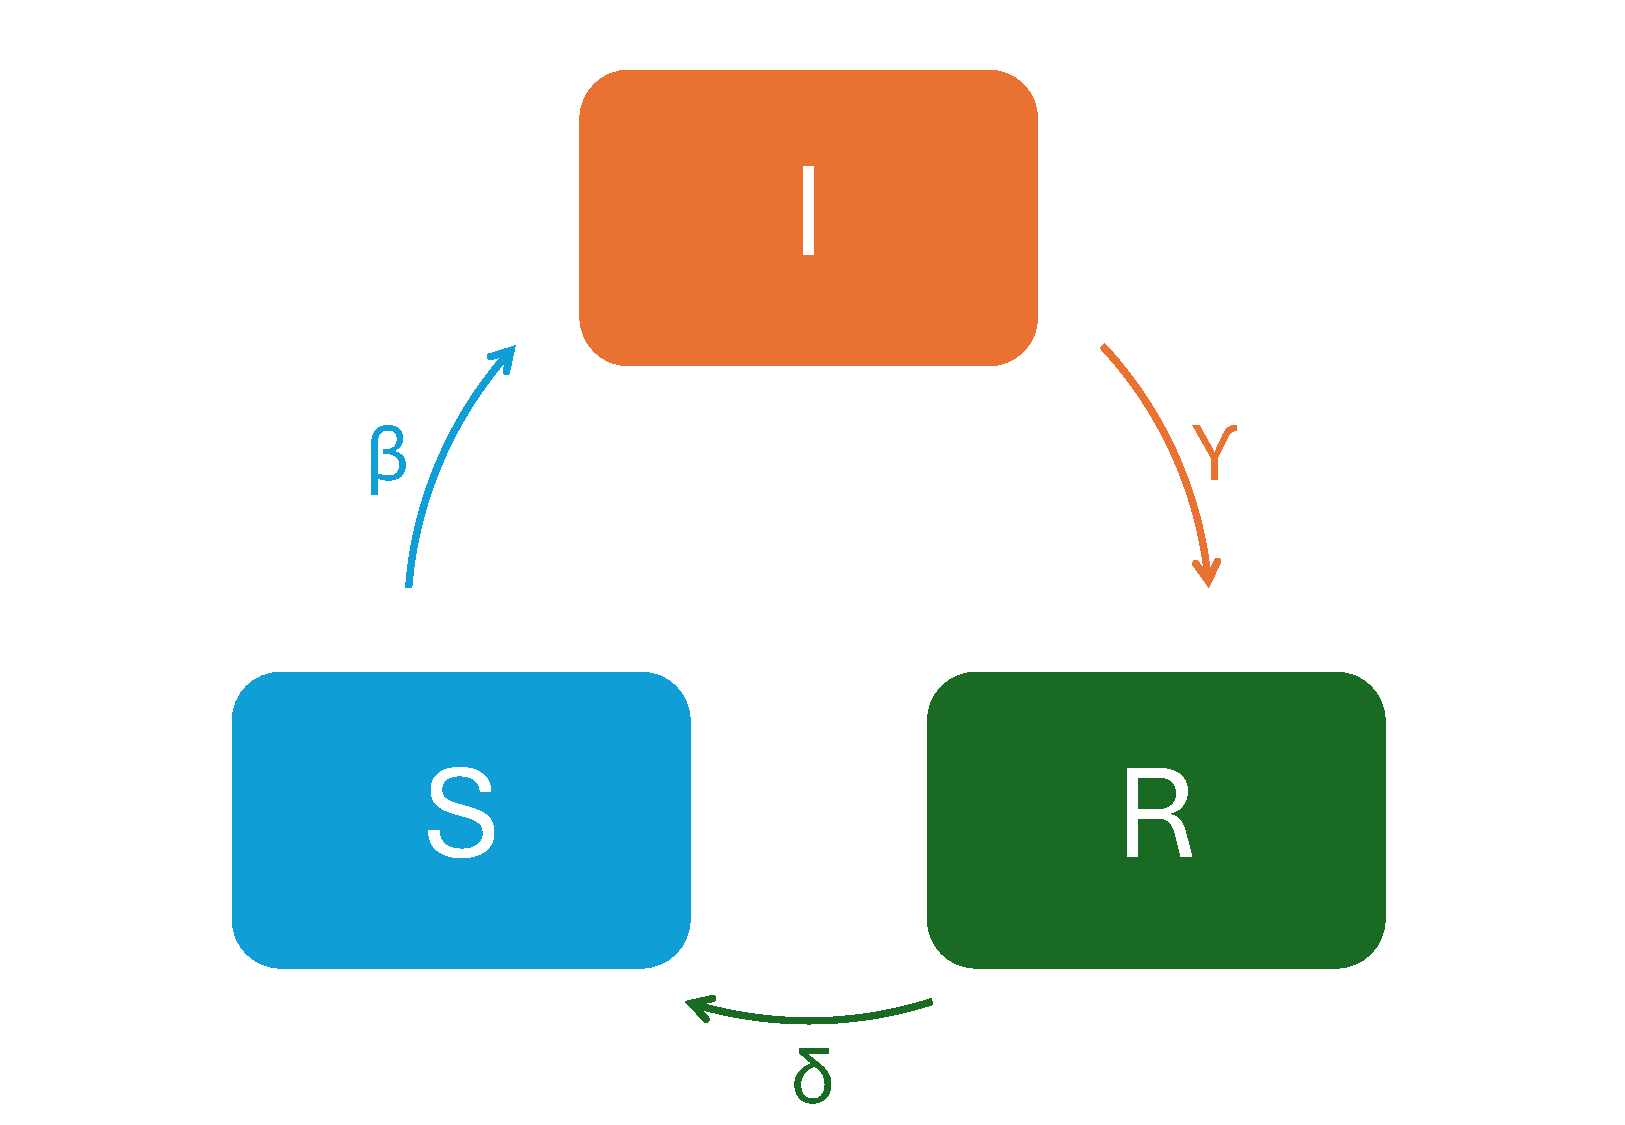
\includegraphics[width=0.65\linewidth]{0_introduction/images_introduction/SIRS_figure_compartmental}
	\caption[SIRS example]{An example of the graph structure of a mean field SIRS model. There are three compartments and the flow rate between them is ruled by the coefficients $\beta$, $\gamma$ and $\delta$.}
	\label{fig:sirsfigurecompartmental}
\end{figure}


\subsubsection{SIR model}
\label{subsec:SIR}
The model that represents the base for epidemic mathematical studying is the SIR.  Here the population or density of individuals is divided into three groups: Susceptible, Infectious, and Recovered. At time $t$ the three groups are identified with the symbols: $S(t)$, $I(t)$, and $R(t)$. 
The symbols used to indicate the density of each group are $s$, $i$, and $r$, while the capital letters are used to specify both the name of the groups or the absolute number of participants in each one. 
Usually, the assumption that N remains stable is made. This is possible considering that the term epidemic identifies a disease with a duration much lower than the life of a person. Considering this assumption the number of deaths and births can be neglected. Alternatively, we can consider that the number of births, which is an influx in the S compartment is roughly equal to the number of deaths, which is an outflux. These statements imply $s(t) + i(t) + r(t)= 1$ and $\dot{s}+ \dot{i} + \dot{r}= 0$.
The disease reproduces horizontal incidence within the population. So, it is the connection with others that causes the infection diffusion. 
$\beta$ is a coefficient that expresses the number of adequate contacts on average of a person per unit of time. The simplest way to explain the meaning of $\beta$ is to consider that not every contact between a susceptible and an infected person can generate a contagion. The formula  $\beta \frac{I}{N} = \beta i$ is then the average number of contacts with infectives per unit time of one susceptible. Finally, the number of new cases per unit of time due to the $S = N s$  susceptibles is $\beta \frac{I}{N} S = \beta N i s$. This form of horizontal incidence is called the standard
incidence. In this incidence, there is no dependence on population size \cite{Hethcote_2000}. This is because the contact of individuals daily is independent of the country dimension in which they live. 

The second transition process in the model is that individuals move from the infectious state to the recovered one at a rate $\gamma$. So the infection duration lasts an average time of $1/\gamma$ days. The $\gamma$ parameter represents the healing or recovery rate of the population. A mathematical interpretation of this term is that  
corresponds to exponentially distributed waiting times in the $I$ compartments. The transfer rate $\gamma I$ corresponds to $P(t) = e^{\gamma t}$. It is the fraction of infected that are still in their class after time $t$ of entering it and with a mean waiting time of $\frac{1}{\gamma}$.


%%
In this initial model, the immunity acquired after recovering from the illness is lifelong. It is equivalent if after being sick a person recovers or dies because it is considered that it will not transmit the infection anymore.  This assumption can be modified and there are often diseases in which after a certain period individuals become again susceptible. Another initial simplification is the one of considers the coefficient $\beta$ and $\gamma$ constant. 

Although the SIR model is quite simple it can predict a very important aspect of an epidemic, the threshold value. This effect was the main novelty studied in the pioneering work of Kermack and McKendrick \cite{kermack1927}. They found that in a fully susceptible population if and only if R0 > 1 an infection can start diffusing. Thus the origin of the term "threshold value" in epidemiology. 

The dynamic of this system has been extensively studied and analyzed during the years CITA. The threshold effect distinguishes between two scenarios. The first is when $R_0 <1 $. It is called "free disease equilibrium. 
In a fully susceptible population, a disease with a $R_0$ less than one does not spread. The initial small number of infected tends to zero and at equilibrium the whole population has remained in the $S$ group. This state, as proved in \cite{Hernandez_Vargas_2022}, is globally asymptotically stable. The second case is when the threshold is larger than one. Here, the number of infected grows until a peak and then decreases to zero. Both this max value of infected and the final number of susceptible can be calculated knowing the system's initial condition ($s_0$ and $i_0$) and the value of $\beta$ and $\gamma$, as explained in \cite{Hethcote_2000}. 
This second scenario analyzed with a simple SIR model permits us to immediately understand how a very aggressive infection can spread across a large part of a population. In this situation, if no countermeasures are taken in time, there can be severe consequences on the society, with social and economic damages. 

\subsubsection{Derivation of I evolution and SIR differential equations presentation}
After having theoretically presented the model, it is now explained one method to derive the mathematical form of the infection compartment evolution. 
The set of differential equations that  describe the dynamic of infection is the following:
\begin{equation}
	\begin{cases}
		dS(t) / dt = -\beta S(t) I(t)\\
		dI(t) / dt = \beta S(t) I(t) - \gamma I(t)\\
		dR(t) / dt =  \gamma I(t)
	\end{cases}
\end{equation}
Here $X(t)$ is indicated as the population at time $t$ in the X compartment. Remember that the assumption of constant population size is also done, so $S(t)+I(t)+R(t) = N$ holds.

The number of infected, with an interval  $\Delta t$, that in a base case can coincide with one day, is given by the equation:
\begin{equation}
	I(t+\Delta t) = I(t) + [\beta S(t)I(t)/N - \gamma I(t)]\Delta t
\end{equation}

If the value of N is large, the variables can be considered as continuous, and imposing a time interval close to zero it becomes:

\begin{equation}
	\frac{d I(t)}{dt} = \lim_{\Delta t \rightarrow  0} \frac{I(t+\Delta t)-I(t)}{\Delta t} = \beta S(t) I(t)- \gamma I(t)
\end{equation}

Consider now the initial state of the system. At the beginning of the disease, considering that there are few infected, the majority of the population is in the susceptible groups, so $S(0) \approx N$. Furthermore, during the initial days of contagion diffusion, this quantity remains stable. Considering this approximation, we have 
\begin{equation}
	\frac{d I(t)}{dt} = (\beta S(0)-\gamma)I(t),
\end{equation} 
which gives now a differential equation with only a variable, $I(t)$, that has a well-known solution:

\begin{equation}
	I(t) = I(0) \exp ^{(\beta S(0)- \gamma)t}
	\label{eqn:sol_I}
\end{equation}



From the analytic solution of the infectious dynamic equation in \ref{eqn:sol_I}, we can see what happens at the beginning of an epidemic.  If the exponential argument has a positive sign it is observed an exponential increase in the number of infected. While, in the opposite case, infected people tend to zero. 
The value $\frac{ \beta}{\gamma} S(0) = 1$ is defined as the epidemic threshold. In the initial phase of the epidemic the relation $\frac{ \beta}{\gamma} S(0) = \frac{ \beta}{\gamma} N $  holds. 
This quantity, normalized, is called the basic reproductive rate, and indicated with the symbol $R_0$.

It measures the intensity of the contagion or the number of secondary infections a sick person can generate. Analysing the equation of susceptibles, with this model we see that it is always decreasing. In the SIR model, if the condition to start the epidemic is satisfied after an increase in the number of Infected, there is a point at which $\frac { \beta}{\gamma} S(0)$ becomes less than one. It is when this happens that the peak of the $I(t)$ curve is reached. Then, the disease begins its falling phase. It is the natural behavior of an epidemic.

\begin{figure}[h]
	\centering
	\subfloat[][\emph{}]
	{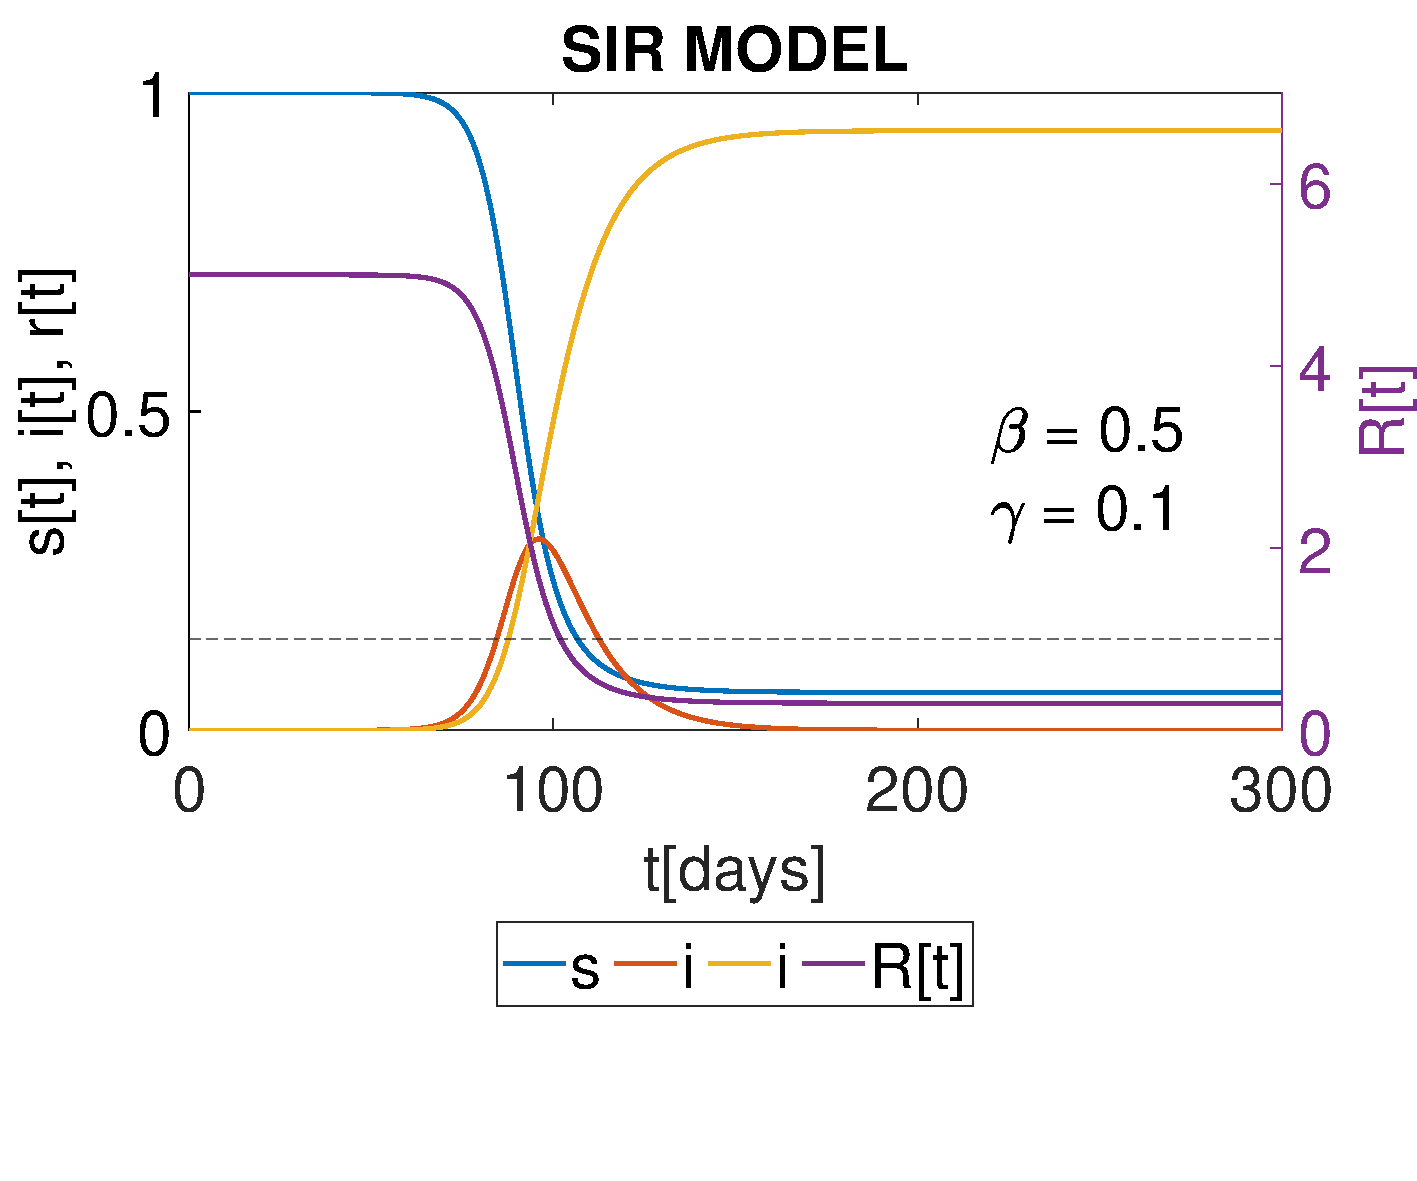
\includegraphics[width=0.48\linewidth]{0_introduction/images_introduction/sir_con_rt}} \quad
	\subfloat[][\emph{}]
	{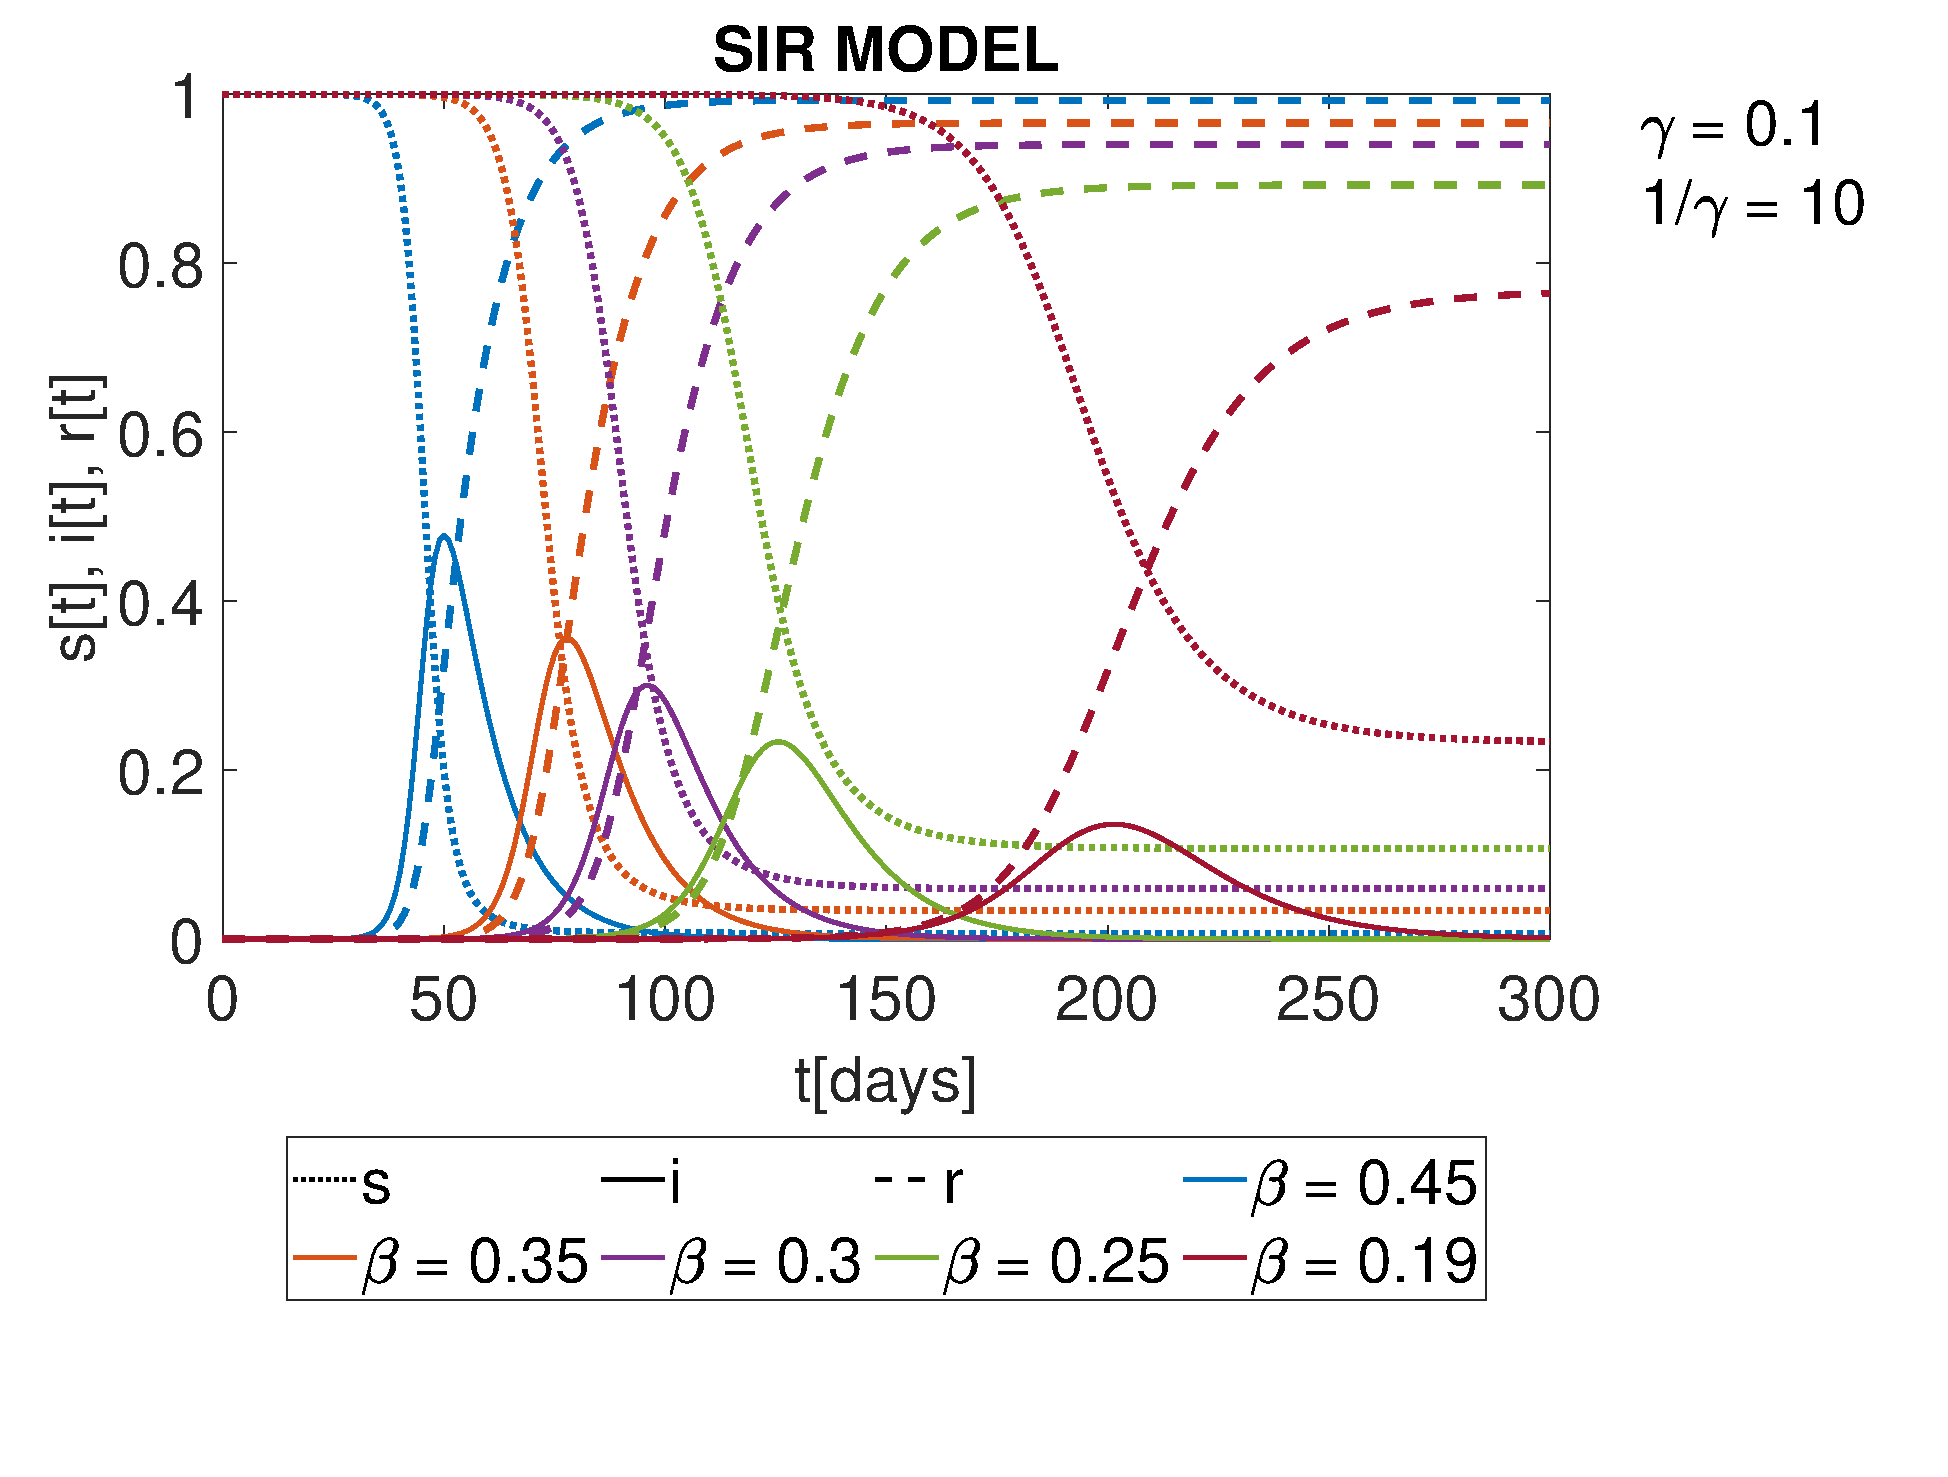
\includegraphics[width=0.48\linewidth]{0_introduction/images_introduction/sir_multipli_beta}} \\
	\caption[SIR dynamic example]{SIR system numerical solutions. Figure a) shows the evolution of compartments in the case of an epidemic. The violet dotted line represents the time-dependent $R_0(t)$. It can be seen that when this parameter is equal to $1$, the number of infected reaches its maximum value. In b) are presented different evolutions of the disease varying only the $\beta$ coefficient. The smaller its value the flattened and the more delayed the infectious curve is.}
	\label{fig:sir_example}
\end{figure}
Other two interesting quantities to consider when a new disease appears are the rate of increase of the infectious and the final size of remaining susceptible at the end of the epidemic. There is a large difference when a population suffers from an epidemic if this ends rapidly because a lot of people get sick or if this number can be controlled, and the infectious curve is flatter. A strategy to flatten the curve can reduce the contact between susceptibles, actuating social distancing or avoiding contact with infected, implementing quarantine measures. These are two simple examples of actions that reduce the value of $\beta$. Another countermeasure is represented by vaccination. Its immediate effect on the epidemic is to remove susceptibles people, so the disease can afflict only a small group and be quickly extinguished. 

\subsubsection{Stochastic models} 	
This is a group of models deriving by the mean-field, but using a different mathematical approach.
In this typology, the transition from one state to another is determined using a function of probability.  Conceptually are derived using the same framework used with ODE models. They are useful when the disease to study has a lower number of infected or if there is a connection between the epidemic outcome and changes in individual dynamics. This is called demographic variability, and it concerns changes in transmission, births, recovery, or deaths within the population. Using stochastic models with Monte Carlo simulations can be useful to investigate epidemic models on networks \cite{Allen2017}. 
The two most important types of models using this approach consider the time variable as continuous, $t \in [0, \infty) $and then the state variable is either discrete (Continuous-Time Markov-Chain) or continuous (Stochastic Differential Equations).
Referring to the SIR model to make a simple example here the S and I compartments are modeled as random variables. The probability of individuals changing groups depends on infection and recovery, the possible events that can occur. It is called transition probability. 
In a Markov chain approach the transition probability is discretized, and there is no dependence on the history of the epidemic to know how it will evolve at time $t + \Delta t$. It is necessary to know only the current state of the process at time $t$. 
In the Stochastic differential equation, the random variables are continuous. 

\subsection{Agent-based networks}

Agent-based models are an alternative technique used to represent disease evolution. This approach is implemented based on the observation of spontaneous connections made by individuals. The evolution of a disease is considered over complex and realistic networks. The focus of this type of model is to understand how the network structure influences the epidemic by observing parameters such as the rate of spread.

In this framework, the nodes of the graph represent individuals (with all the properties that the modeler deems relevant for the study), while the edges represent interactions between people. Nodes can also represent subgroups of people, and using weights on edges makes it possible to characterize the strength of these interactions.

An advantage of this type of model is that it offers a very intuitive approach to epidemic modeling. Using an individual perspective guarantees an immediate interpretation of the model. A precise agent-based model can provide a greater understanding of the illness under consideration and direct information about countermeasures to implement to stop or mitigate its spread. However, to be powerful and capable of performing good analyses and predictions, a lot of information must be integrated into the model. Only if the agent-based model is highly capable of realistically reconstructing a real network can it be a reliable instrument, and achieving this requires very complex work.
\begin{figure}
	\centering
	
\includegraphics[width=0.5\linewidth]{0_introduction/images_introduction/agent_based}
	\caption[Agent based network representation]{Agent based network representation}
	\label{fig:agentbased}
\end{figure}

%%

An example of a possible mathematical implementation of this class of models is now briefly presented. One possible technique to describe peer-to-peer contact in a graph structure is realized through a probabilistic framework. Here, assuming a total of $n$ agents in the model, spread processes can be described as a function of probability. Using Markov processes, each agent has a certain probability of transitioning from one state of the disease to another. To calculate the value of these probabilities, both the information derived from the network structure and parameters related to the disease, such as infectivity and recovery rates, are used. In this way, a stochastic evolution model of the processes is developed.

Considering an SIS model described with a Markov process: it has a dimension of $2^n$, while implementing an SIRS model requires a dimension of $3^n$. Because the size of models developed in this manner becomes rapidly enormous, a mean-field approximation is employed. It is based on the assumptions of a network composed of a sufficiently large number of agents and on the independence of these nodes. With this technique, by taking expectations, the transition rates of individuals are approximated. Using these approximations, the boundary values of the agent's probability of infection can be determined at each time step \cite{Hernandez_Vargas_2022}.

\subsection{Multilayer systems and networks} 

The complex dynamic of interactions existing in the real world, develops in multiple patterns, with complicated relationships. This connection can change over time, and using the theory of multilayer systems it can improve the comprehension of such complexity. Additional information can be added to the model, for example, different types of interactions, like physical contact or information sharing, time dependency coefficients, or reliance between different parameters in nature, creating cause-effect relationships. 
It is a more recent development of the research, the traditional network theory was revisited, to create a framework that can include multiple networks, that evolve and influence each other \cite{DeDomenico2016} and can be helpful to manipulate complex systems like human relationships. Some interesting results obtained are the possibility that the onset of one disease can depend on the onset of the other one. There can be regimes in which the criticality of the two dynamics is interdependent and others in which the critical effect is only one-directional \cite{DeDomenico2016}. 
One possible way to develop models with this structure is to imagine that each layer represents a different type of interaction. An epidemiological example is a layer in which the physical contact between people is simulated and another represents social structure, the network of relations that every person has. This instrument provides a natural representation of coupled structure and dynamical processes. It has been presented in multiple works in the past years, for example in CITA. 
The dynamic realized in multiple systems can be single or coupled. In the first, there is a top layer with its dynamic evolution running on top of a multilayer network. The coupled structure instead is the one in which the phenomena described in each layer evolve with the influence of what is happening in the other. 
Multilayer networks have multiple dimensions of connectivity, called "aspects" and they have to be considered simultaneously. 
They can also be considered with two different mathematical structures. 
\begin{figure}[]
	\centering
	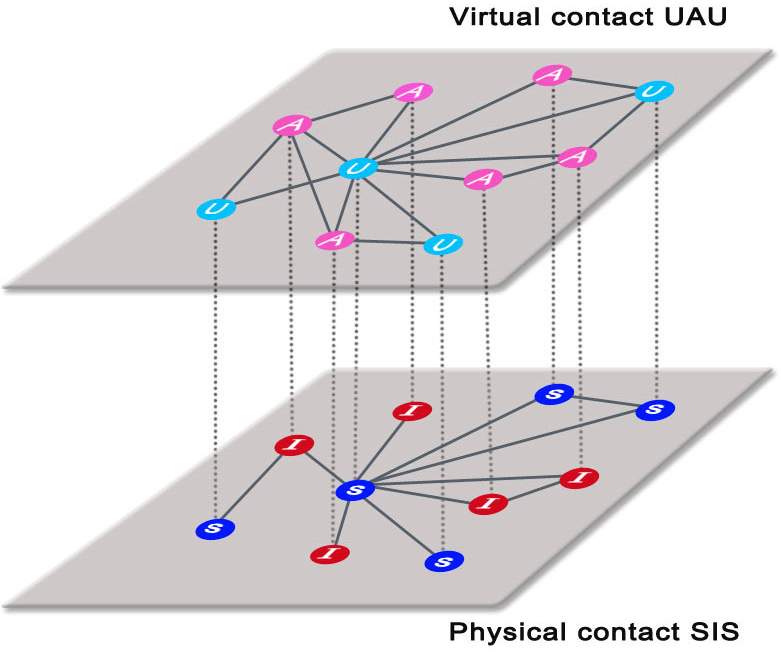
\includegraphics[width=0.6\linewidth]{0_introduction/images_introduction/multi_layer}
	\caption[Multi-layer network]{Representation of a multiplex structure. The figure is taken by the work of \cite{Granell2013} and shows the network implemented in their model. There is an awareness and an epidemic layer. In this case, the node connected with the interlayer connection represents the same individual.}
	\label{fig:multilayer}
\end{figure}

The first uses the same set of compartmental structure and mean-field models presented in the section before \ref{subsec:mean_field}. Here, from a mathematical point of view, there is no such difference in the manipulation and analysis of the system. The distinction relies on the meaning of the compartments and parameters created and on the dependence of the coefficients, which can be time and state-dependent.

The second option considers an agent-based structure. Here, considering a graph structure, composed of nodes and links between them, it is possible to classify three types of edges:
\begin{itemize}
	\item intra-layer edges, the connection of nodes on the same layer.
	\item inter-layer edges, the connection between a replica of the same node, but lying on a different layer of the structure;
	\item inter-layer edges, but coupling nodes representing distinct entities. 
\end{itemize}

A possible representation is done using a $4^{th}$ order tensor or coupling a set of adjacency matrices, called "supra-adjacency matrices". The feature that can be studied is the structural properties of the network, depending on how the various layers are coupled together. The presence of clusters or most central nodes is also important.
\chapter{Main objectives and summary of the contents}

 In this section, the main objectives pursued with the present thesis work are presented and it is described the composition of the thesis text. 

\chapter{Review of epidemiological behavioural and opinion models in literature}

The development of a epidemiological model, that can capture the evolution of a disease influenced by the behaviour of individuals, begins from a study and review of the most significant works already present in this research topic.
These are the different main type of model that have been investigated:
\begin{itemize}
	\item deterministic/mean field models
	\item opinion models
	\item multilayer networks
	\item opinion-disease models	
\end{itemize}

Now it is presented for each of them, the main aspect and knowledge, useful for the development of my model.   

\section{Opinion models}
In the analysis performed by Wang \cite{Wang_2019}, are presented mechanism implemented to explain co-evolution spreading in complex network. The principal methodologies created over time are threshold model, that can use a linear threshold or a “Watts threshold”. Here each node has a random different threshold, based on a certain distribution. Using a threshold means that a node change opinion on the basis of its neighbours’ belief. The shape of the network is then fundamental for an opinion to spread. The best scenario is the one in which there is a low degree of randomness, and the network is regular. Also, cluster can have a reinforcement effect, if they are sufficiently connected to the resto of the graph. Their work then report analysis based on competition or cooperation of opinions “contagions”. And a SAR model is presented. Similar to a SIR, here the meaning of letter A is “adopted”. It means becoming convinced of a certain opinion, but with a probability or rate to then return to the previous behaviour. Also the work of \cite{Nunner2021} define and test some different models based on trade-off between the benefit of having connections and the penalty for acquiring infections. It is showed that when the behaviour of people depends on maximizing their net benefit, the individual risk perception plays an important role in the formulation of a cost function. The models derived with this so called co-evolutionary approach, have an overall dynamic very correlated between the two strati: it is a feedback loop between infection spreading, people behaviour adaptation and consequently structural modification in the network.


\section{Multilayer network}
One work based on feedback between two networks concatenated is the one performed by Peng et all, \cite{Peng2021}. Here there is explained a model based on two graphs, where one simulates the evolution of a disease, using a SIR or SIRS dynamic, and another explicit the behaviour of individual in a UPAU network. U means uninformed, P pro-physical distancing and A anti-physical distancing.  In this network the people’s conduct influence the $\beta$ coefficient of the epidemic diffusion. They demonstrate the effectiveness of having an opinion in reducing the negative effect of a disease and that lengthening the duration time for which an individual maintains opinion can help suppressing the transmission.
Study the effect of competition in a multilayer network is the objective of Teslya et all research \cite{teslya2022}. At cause of interpersonal communication individual can change their opinion. They are divided in two main groups, positive or negative w.r.t health conduct. Here is also inserted an influence due to assortatively when contacting with others. Their principal results further than the fact that opinion influence disease, is realizing a model in which the two opinions can coexist at equilibrium. There can be oscillation of prevalence due to increased transmissibility of infection. In SIR model they demonstrate a reverse correlation between the rate of social contact and the peak magnitude of infectious. The causes of oscillations in the disease dynamic are a high infection rate and a pronounced difference in infection rate between individuals with different opinions. The others important factors are the high-rate opinion exchange and high sensitivity of population to prevalence. 
In the article \cite{ Alvarez_Zuzek_2017} the opinion about vaccination is taking in consideration, into a SIR+V mean field model. Conversating is the mean used by individual to modify their opinion. With a very positive opinion susceptible individuals can choose to take the vaccine. Interesting they use a r factor to describe the extremism in opinion. Varying this coefficient, they observe that the best scenario for delay the development of an epidemic is the one where the society is neutral. So, when there aren’t compromise or persuasion, but the conversation is based on “rational” arguments.  Another works analysing two competing opinion is \cite{Epstein_2021}. Here population is sensitive to both fear of vaccine and disease. These two interact and the vaccination grow rate increases only if the fear of the disease is larger than the of vaccine.  The infection curve is very influenced by the presented dynamic, and the best scenario is obviously the one in which the fear of vaccine does not exist. However, in the case where the two fears coexist there is an improvement in the number of infected, for multiple infection waves.
The work by Auld \cite{Auld_2003}, reflect an observed characteristic in society: pessimistic expectations over the future induce a more risky behaviours. This conclusion derives observing and simulation evolution correlated to the news about a vaccine. This knowledge causes a decrease in infection rate before the vaccine becomes available. Then there is a return to normal behaviour. If there are not information, pessimism cause more risky behaviour. 
In \cite{Sontag_2022} there is another SIR and opinion model, with population that is divided in trusting and distrusting. They add in the model the effect of fading and a global force, that simulates central interventions. The main interesting conclusion of their work is that strong public intervention have a similar effect to the network to the ones obtained if the population is composed of trusting and compliant individuals. However, higher percentages of distrusting cause the model to pass a phase transition where outbreaks cannot be suppressed. 
A different approach in using a multilayer network is the one realised in \cite{Turker_2023}, where the social structure of a town is re-created. Every layer describes the places populated by individuals: from house, to work, distinguishing between different type of work, and considering a level for friendship. Each person is present to more than a layer and, in each layer, relates to different agents, based on the social group’s provenience.  Using this approach, they have found that the level in which is easier for an outbreak to develop is the one associated with friendship. Here the interaction is closer with others, the security level is lower. For this reason, a lower value of transmissibility rate $\beta$ is sufficient to have an epidemic with many susceptible involved. 

\section{Opinion-disease model}
The work done by Funk and its colleagues \cite{ Funk_2010}, it is very interesting: they collect and explain systematically the behavioural reaction of population in response to a pandemic. They classify the human behaviour subject to different possible sources of information. An information can be global available or local. This reflects the way it radiates or if develops in social cluster. Another important difference is related to objectivity. Certain information is based on belief and can change with time. This typology can be influenced by the social connections of an individual or by the influence of external agents, like media. Cognitive bias also can have an impact on our opinions: amplification, confirmation, anchoring bias. They then focus on the influence of self-initiated action in the control of disease diffusion. When an individual change its behaviour, form a modelling point of view this can influence: its probability to change state (from S to I for example). The value of $\beta$ or $\gamma$. Modification in the contact network, with a self-isolation or adherence to more cautious conduct. Fear has an important role in how people face epidemic. Due to this emotion, people can decide to get vaccinated for example (or not, if they are more frightened by vaccines). Another phenomenon observed and influenced by fear is saturation. When there is many infectious people tend to decrease their number of contact and this cause a decrement in the I curve.  Another multilayer network with two opinion, 0 where individual not take precautions and 1 where the protective measures are used, is presented in \cite{Frieswijk_2022}. This model is associated to a SIS disease one. The article studies the stability of asymptotically equilibria of the system. Assuming different value of a parameter used to describe risk perception they found a set of final possible states. The most interesting is a stable asymptotical equilibrium in which there is a periodic epidemic outbreak and a consequently population behaviour response, changing behaviour to a safer.
An analysis of people choices about vaccinations is done by \cite{Bauch_2012}, they study the feedback between the positive effect due to vaccination and the fear of being vaccinated. In fact, thanks to vaccines, the disease incidence can become very low, and the perception of risk related to them can seem larger. They implemented an approach based on game theory and using social learning.
A possibility to integrate the effect of opinion in the dynamic of an epidemic, is creating different subgroups of susceptible. They are separated according to their level of opinion, and the less they belief in use of NPI, for example, the higher probability of being infectious they have. This is the approach used in \cite{Tyson_2020}. They also implemented different functions describing the influence between opinion and the possibility to become infected. 
The influence of media has also been analysed. This is interesting, because it’s a communication channel that can be used by government, and so it is an available control measure that can be implemented, to try control the behaviour of population.  For example in \cite{Collinson2014} a parameter depending on I value simulates the effect of media covering the news about the disease. Increasing the number of infectious cause, the creation of news and other media about it. These can have as effect to induce more people practice social distance for example. Study both the effect of media, see as a central node of communication joined with opinion evolution is done in \cite{Granell_2014}. Nodes co-exist into two layer, one for disease spreading and one for awareness, (unaware-aware-unaware model). In their application the awareness process without media, must reach a certain level on the transmissibility of awareness to influence the onset of epidemic. Instead, with an influence of media, greater than zero, this “metacritical” point disappears. A central broadcast, even with a small communication influence power, as a direct effect on all the network dynamic. 

